%!TEX root = ../dissertation.tex
\externaldocument{../frontmatter/abbr}
\begin{savequote}[75mm]
    If it looks like a duck, and quacks like a duck, we have at least to consider the possibility that we have a small aquatic bird of the family Anatidae on our hands.
\qauthor{Douglas Adams}
\end{savequote}
\chapter{Progetto di stage}
\label{chap2}
\section{Approfondimento del contesto}
\subsection{Contesto di sviluppo}
\label{sec:devctx}
La piattaforma fa parte di un ecosistema già esistente di servizi per la salute, fruibili presso farmacie affiliate. Esiste, quindi, come parte di un insieme di applicativi paralleli e ne condivide il database e parte della codifica: questo documento si limiterà a descrivere i moduli, le classi e le funzionalità realizzate o adattate per l'implementazione della piattaforma ``Biota''.
L'applicativo si compone di una parte \textit{back end} (in esecuzione su un server dedicato) e una parte \textit{front end} (eseguita all'interno del browser dell'utente) sviluppate separatamente e integrate grazie all'uso di \ref{itm:api} specifiche; obiettivo dello stage è stata la realizzazione del primo, in modo funzionale all'utilizzo con il secondo. La tecnologia principale, descritta più avanti nel documento, è Ruby on Rails 5 (\textit{framework} per lo sviluppo di applicativi web).

\subsection{Caratteristiche degli utenti}
``Biota'' prevede l'utilizzo da parte dii utenti autorizzati con diversi permessi: farmacisti, gastroenterologi e supervisori del laboratorio. Tutte le categorie di utenti autorizzati eseguono il \textit{login} nella piattaforma allo stesso modo, ma ad ognuno viene mostrata un'interfaccia con diverse funzionalità. Il cliente non fa parte degli utenti autorizzati in quanto non può accedere direttamente alla piattaforma, e tutte le operazioni che lo coinvolgono sono supervisionate dal farmacista.
Per quanto riguarda il pannello amministrativo, ne è previsto l'utilizzo da parte di utenti autorizzati registrati separatamente; tali amministratori fanno parte della società che gestisce la piattaforma. Per interazioni con servizi esterni sono inoltre disponibili delle \ref{itm:api} \ref{itm:rest}, utilizzate principalmente per l'integrazione con il gestionale del laboratorio di analisi. 

\subsection{Contesto di utilizzo}
Il flusso operativo previsto è il seguente: il cliente richiede al farmacista di effettuare un esame, e inserisce i propri dati registrandosi alla piattaforma; il farmacista quindi ottiene il consenso al trattamento dei dati e fa compilare un breve questionario al cliente, consegnando un kit per il prelievo del campione di materia fecale. Questo viene poi restituito, registrato al cliente ed inviato al laboratorio previa prenotazione della spedizione: grazie alla corrispondenza univoca tra il codice identificativo del campione e la sessione associata all'esame, è garantito l'anonimato del cliente. Il laboratorio, ricevuto il campione, ne effettua il check-in nel proprio gestionale (aggiornandone automaticamente lo stato nella piattaforma) e procede alle analisi necessarie. Viene quindi inviato il referto delle analisi insieme a dei dettagli aggiuntivi, che viene reso disponibile nella piattaforma al gastroenterologo affiliato che aggiunge la sua diagnosi e la dieta consigliata. Dopo un'ulteriore controllo ed eventuali modifiche da parte di un supervisore del laboratorio, il referto completo può essere generato e reso disponibile al cliente \textit{on-demand}, concludendo la procedura.

L'accesso al pannello amministrativo consente di creare, distruggere e modificare alcune categorie di record del database, come ad esempio le varie tipologie di utenti o le farmacie affiliate. Esso viene utilizzato principalmente per l'inserimento di nuovi utenti autorizzati, il recupero di informazioni rilevanti quali il consenso al trattamento dei dati, e per la risoluzione di problematiche grazie all'accesso privilegiato al database.

\section{Definizione degli obiettivi}
Nella seguente sezione verranno esposti in via generale gli obiettivi e requisiti che l'applicativo realizzato doveva soddisfare. È importante notare che, data la natura agile del metodo di lavoro impiegato dall'azienda, gli obiettivi presentati nel piano di lavoro sono stati soggetti a modifiche e aggiunte di lieve e media entità; per completezza e possibilità di confronto, di seguito verranno esposti sia i requisiti iniziali che quelli elaborati a fronte dell'interazione con il cliente.
\subsection{Notazione}
Si farà riferimento agli obiettivi definiti secondo la seguente notazione:
\begin{itemize}
    \item \textbf{O} indica un obiettivo obbligatorio, vincolante in quanto requisito primario stabilito dal committente.
    \item \textbf{D} indica un obiettivo desiderabile, non vincolante o strettamente necessario, ma dal riconoscibile valore aggiunto.
    \item \textbf{F} indica un obiettivo facoltativo, rappresentante un valore aggiunto non necessariamente competitivo.
\end{itemize}
\vspace{-12pt}
\subsection{Piano di lavoro}
Il piano di lavoro, stilato in collaborazione con il relatore ed il tutor aziendale nella settimana precedente all'inizio dello stage, espone una serie di requisiti emersi dalle esigenze del cliente emerse in fase di avvio del progetto.
\subsubsection{Obiettivi}
\paragraph{Obbligatori}
\begin{itemize}
    \item \underline{O01}: Analisi ed implementazione \ref{itm:api} \ref{itm:rest} laboratorio
    \item \underline{O02}: Analisi ed implementazione \ref{itm:api} GraphQL per il flusso operativo base
\end{itemize}
\vspace{-12pt}
\paragraph{Desiderabili}
\begin{itemize}
    \item \underline{D01}: Analisi ed implementazione di test dei sistemi di pagamento e fatturazione
    \item \underline{D02}: Suite di testing del software prodotto
    \item \underline{D03}: Documentazione completa
\end{itemize}
\vspace{-12pt}
\paragraph{Facoltativi}
\begin{itemize}
    \item \underline{F01}: Ulteriori modifiche all’applicazione che esulano da quando riportato nel piano di lavoro
\end{itemize}
\vspace{-12pt}
\subsection{Modifiche al piano}
Durante il corso dello stage, nello svolgimento del ruolo di Product Owner da parte del tutor aziendale, ci sono state varie interazioni con il cliente che hanno portato a ridefinire alcuni requisiti desiderabili e a specificare in modo più preciso i requisiti facoltativi. Tali modifiche sono sempre state fatte in accordo alle possibilità di soddisfazione entro i tempi previsti, e tenendo in mente che la piattaforma sarebbe entrata in produzione al completamento delle funzionalità per l'esecuzione flusso di attività base.
\subsubsection{Obiettivi rivisti}
\label{sec:reqs}
\paragraph{Obbligatori}
\begin{itemize}
    \item \underline{O01}: Analisi ed implementazione \ref{itm:api} \ref{itm:rest} laboratorio
    \item \underline{O02}: Analisi ed implementazione \ref{itm:api} GraphQL per il flusso operativo base
    \item \underline{O03}: Adattamento e rafforzamento del codice esistente
\end{itemize}
\vspace{-15pt}
\paragraph{Desiderabili}
\begin{itemize}
    \item \underline{D01}: Generazione PDF con informazioni specifiche
    \item \underline{D02}: Suite di testing del software prodotto
    \item \underline{D03}: Documentazione completa
    \item \underline{D04}: Registrazione del consenso al trattamento dei dati
\end{itemize}
\vspace{-15pt}
\paragraph{Facoltativi}
\begin{itemize}
    \item \underline{F01}: Autenticazione mediante HMAC
    \item \underline{F02}: Ulteriori modifiche all’applicazione
\end{itemize}

\section{Pianificazione delle attività}
Il piano di lavoro prevedeva anche una suddivisione settimanale delle attività dedicate alla realizzazione del progetto, distribuendo le 300 ore previste su un periodo di 8 settimane, più una settimana di \textit{slack} per accomodare eventuali impegni accademici.

La suddivisione settimanale prevista era la seguente:
\begin{itemize}
    \item \textbf{Prima settimana (20 ore)}: Comprensione del sistema e degli obiettivi;
    \item \textbf{Seconda settimana (40 ore)}: Analisi dei requisiti;
    \item \textbf{Terza settimana (40 ore)}: Studio e setup ambiente di sviluppo, progettazione;
    \item \textbf{Quarta settimana (40 ore)}: Implementazione;
    \item \textbf{Quinta settimana (40 ore)}: Implementazione;
    \item \textbf{Sesta settimana (40 ore)}: Implementazione;
    \item \textbf{Settima settimana (40 ore)}: Implementazione, test e validazione;
    \item \textbf{Ottava settimana (40 ore)}: Test e validazione, documentazione.
\end{itemize}
\vspace{-5pt}
\begin{table}[h]
    \begin{center}
        \begin{tabular}{|c|c|}
          \hline % linea orizzontale
          \hspace{5pt}\textbf{Attività}\hspace{5pt} & \textbf{Monte ore}  \\\hline
          Comprensione sistema e obiettivi & 20 \cr\hline
          Analisi dei requisiti & 40 \cr\hline
          Progettazione  & 20 \cr\hline
          Studio e setup ambiente di sviluppo &  20 \cr\hline
          Implementazione &  150 \cr\hline
          Test e validazione &  30 \cr\hline
          Documentazione &  20 \cr\hline\hline
          \textbf{Totale} &  300 \cr\hline
        \end{tabular}
        \caption{Totale di ore dedicato a ciascuna attività.}
        \label{tab:ore}
    \end{center}
    \end{table}

    
\begin{figure}[h!]
    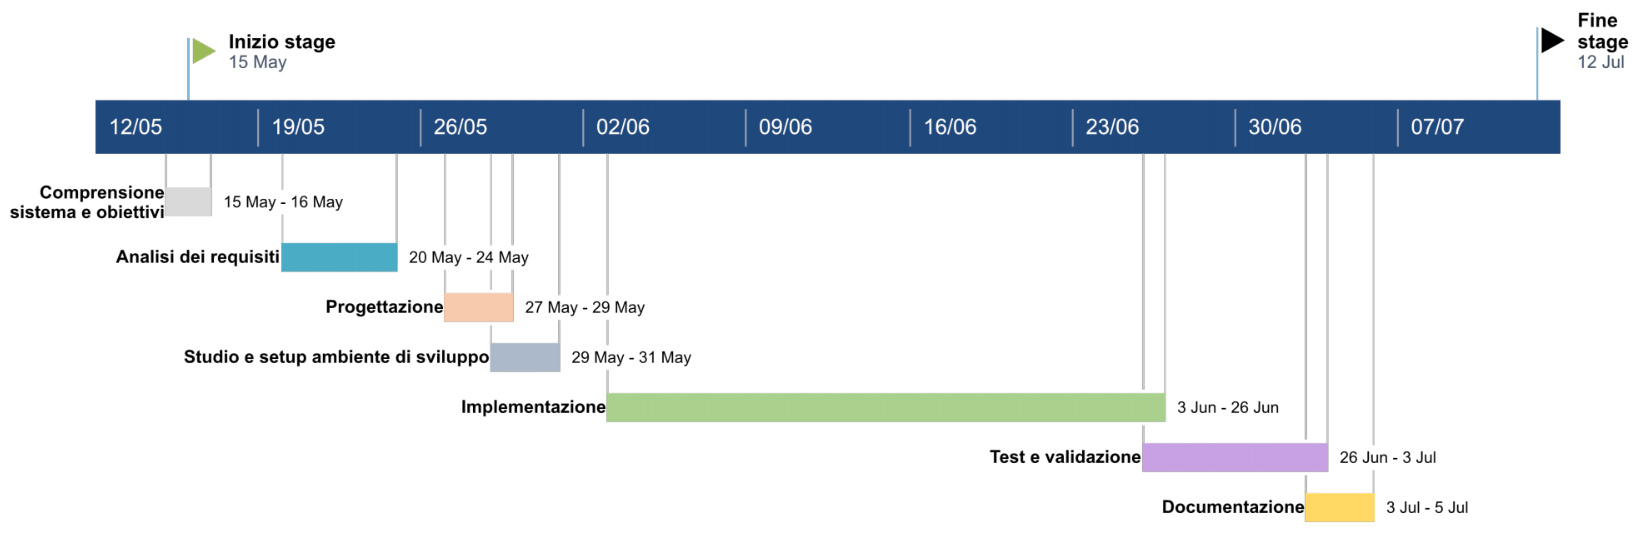
\includegraphics[width=\textwidth]{figures/gantt.png}
    \caption[Diagramma di Gantt di pianificazione delle attività]{Diagramma di Gantt di pianificazione delle attività.
    \label{fig:gantt}}
\end{figure}    

\section{Tecnologie utilizzate}
Di seguito vengono discusse le tecnologie individuate per la realizzazione del progetto. Alcune di esse, quali Ruby on Rails e RubyMine, sono state richieste dell'azienda; altre (principalmente gemme per Ruby) sono state ricercate e proposte dal laureando per soddisfare alcuni dei requisiti individuati.

\subsection{Ruby}
\begin{figure}[h!]
    \centering
    
\includegraphics[height=2.5cm]{figures/ruby.png}
    \caption[Logo di Ruby]{Logo di Ruby.
    \label{fig:ruby}}
\end{figure}
Ruby è un linguaggio di programmazione ad alto livello, interpretato, e orientato agli oggetti con paradigma puro: ogni componente del linguaggio è trattato come un oggetto. 

Alcune tra le caratteristiche più rilevanti di Ruby sono la presenza di tipizzazione dinamica, \textit{garbage collector} e \textit{duck typing} (``Se sembra un'anatra, nuota come un'anatra e starnazza come un'anatra, allora probabilmente è un'anatra.''), ovvero il poter considerare l'insieme dei metodi di un oggetto anziché il suo tipo per decidere se è valido a \textit{run-time}.

Si tratta un linguaggio molto flessibile che offre grande libertà allo sviluppatore e supporta pratiche come il \textit{monkey patching} (ridefinire una classe in un punto diverso dalla definizione originale) e la ridefinizione di metodi a \textit{run-time}.
Esiste una grande varietà di programmi e librerie Ruby, noti come ``gemme'', il cui utilizzo verrà discusso in seguito.    
\subsection{Gemme}
Le gemme sono librerie e programmi Ruby distribuiti sotto forma di pacchetti in modo non dissimile dai moduli in Node.js: l'installazione è gestita dal \textit{package manager} RubyGem, individualmente tramite terminale (con il comando \texttt{gem install nome\_gemma}) oppure di gruppo specificando le gemme desiderate nel file \texttt{Gemfile}, che viene automaticamente letto da RubyGem con l'esecuzione del comando \texttt{bundle install}.

\subsubsection{AWS SDK for Ruby}
Insieme di gemme che facilitano l'interazione con i servizi web di Amazon, fornendo classi e metodi ad-hoc; l'\ref{itm:sdk} è suddiviso in moduli specifici per ogni servizio, permettendo di scegliere quali gemme usare a seconda delle necessità, e di aggiornare le gemme utilizzate in modo indipendente. In particolare è stata utilizzata la gemma \texttt{aws-sdk-sns} per l'invio di SMS tramite Amazon Simple Notification Service.

\subsubsection{Database Cleaner}
Gemma di supporto all'esecuzione dei test, offre varie strategie di pulizia di un database per il testing di una applicazione in Ruby. Il caso d'uso principale di questa gemma è l'assicurare di avere un database pulito prima di eseguire i test e di non avere record residui dopo ciascun test, in modo da non avere interferenze nei risultati. Supporta il \ref{itm:dbms} PostgreSQL.

\subsubsection{Factory Bot}
Gemma di supporto alla realizzazione di test, permette di definire la procedura di creazione di oggetti complessi attraverso metodi a cui passare pochi parametri (detti \textit{factory}). Definire una \textit{factory} per una classe consente di richiamarla in seguito per generare nuove istanze di quella classe, con attributi generati casualmente o specificati manualmente. Factory Bot offre molte altre funzionalità, quali la possibilità di definire vari \textit{trait} (collezioni di attributi assegnati in un modo specifico) per la creazione di un oggetto e di introdurre ereditarietà tra \textit{factories}. È stato scelto di usare questa gemma in quanto permette di realizzare facilmente istanze di \textit{models} di Rails replicandone anche le relazioni con altri \textit{models}. 

\subsubsection{HexaPDF}
Libreria che permette interazioni ad alto e basso livello con file \ref{itm:pdf}: è possibile leggere e modificare il codice sorgente di un documento, oppure sfruttare i \textit{wrappers} presenti per effettuare operazioni ad alto livello come l'inserimento di immagini o figure. Utilizzata per la generazione dinamica di referti.

\subsubsection{Jbuilder}
Jbuilder è una gemma molto utile che fornisce un \ref{itm:dsl} per dichiarare strutture \ref{itm:json} anche complesse, utilizzando strutture \textit{if/else} e cicli. Un file \texttt{.jbuilder} contiene la dichiarazione di una struttura dati \ref{itm:json} che, al momento del \textit{rendering} da parte di un \textit{controller} di Ruby on Rails, viene elaborata e generata secondo i dati disponibili. Questa gemma è stata utilizzata per generare i body delle risposte HTTP date dai \textit{controller}, data la necessità di utilizzare strutture ricorsive.

\subsubsection{ROTP}
Acronimo di ``Ruby One Time Password'', questa gemma permette di generare e verificare codici \ref{itm:hotp} e \ref{itm:totp} in accordo agli standard RFC 4426 \footnote[1]{http://tools.ietf.org/html/rfc4226} e RFC 6238 \footnote[2]{http://tools.ietf.org/html/rfc6238}. ROTP è inoltre compatibile con Google Authenticator su dispositivi Android e iOS. La gemma è stata sfruttata per verificare il consenso al trattamento dei dati mediante codici TOTP inviati per SMS.

\subsubsection{RSpec}
Framework di \textit{behavior-driven development} per Ruby, RSpec è un \textit{tool} per la creazione di test per codice Ruby. RSpec fornisce un \ref{itm:dsl} molto intuitivo e descrittivo per la realizzazione dei test, permettendo di definire precisamente i vari scenari in cui si desidera verificare il comportamento del codice. Il funzionamento di base di RSpec si basa su ``esempi'' e ``aspettative'': un esempio è un particolare scenario che si desidera testare, e le aspettative descrivono lo stato che il codice dovrebbe raggiungere ad un certo punto della sua esecuzione.
RSpec, in congiunzione con altre librerie di supporto, è stato utilizzato per realizzare la suite di test per l'applicativo.

\subsubsection{RuboCop}
Gemma per l'analisi statica e la formattazione del codice, basata sulla \textit{style guide} della community di Ruby. RuboCop permette di scansionare il codice rilevando errori e segnalandoli allo sviluppatore; per errori comuni è anche disponibile una funzione di correzione automatica.

\subsubsection{Shoulda Matchers}
Gemma di supporto alla creazione di test, semplifica di molto la creazione di nuovi esempi con RSpec fornendo una sintassi più sintetica per le aspettative. È stata utilizzata nel progetto per rendere i test più leggeri, leggibili e veloci da realizzare.


\subsection{Ruby on Rails}
\label{sec:2.2.3}
\begin{figure}[h!]
    \centering
    
\includegraphics[height=2.5cm]{figures/rails.png}
    \caption[Logo di Rails]{Logo di Rails.
    \label{fig:rails}}
\end{figure}
Per la realizzazione del progetto Moku ha scelto di usare Ruby on Rails 5 (noto anche come Rails), un \textit{framework} \textit{open source} per applicativi web realizzato in Ruby e utilizzato da celebri siti come GitHub (servizio di hosting per \textit{repository} Git), Twitch (servizio di \textit{live streaming}) e SoundCloud (piattaforma di distribuzione musicale). Rails è stato scelto per la caratteristica di velocizzare notevolmente lo sviluppo di nuovi applicativi, rimuovendo le parti "ripetitive": ad esempio offrendo alias concisi per operazioni di base (e.g. iterazioni su collezioni di oggetti, strutture if/else) che riducono la verbosità del codice.

I principi cardine di Rails sono due:
\begin{itemize}
    \item\textbf{Do not Repeat Yourself}: il principio \ref{itm:dry} sostiene che vadano evitate tutte le forme di ripetizione e ridondanza logica nell'implementazione del software; ad esempio, non è necessario specificare le colonne della tabella del database nella definizione di una classe, in quanto Rails recupera automaticamente tale informazione.
    \item\textbf{Convention over Configuration}: il principio \ref{itm:coc} sostiene che il programmatore dovrebbe esplicitare solo le parti ``non convenzionali'' del codice; ad esempio in Rails esiste per convenzione una corrispondenza tra il nome di una classe e il nome di una tabella del database, quindi essa non va specificata.
\end{itemize}
\vspace{-25pt}
\subsubsection{Integrazione tra i componenti}
Rails è un \textit{framework full-stack}, ovvero offre tutti i componenti richiesti per lo sviluppo di un applicativo web, nativamente integrati tra di loro: tramite l'uso di script per la creazione di file, detti \textit{generators}, è possibile creare contemporaneamente sia una tabella del database che la classe corrispondente; essi sono automaticamente associati tramite convenzioni di nomenclatura. 

Il database, indipendentemente dall'implementazione, può essere modificato tramite \textit{migrations}, istruzioni per la modifica dello schema da parte di Rails. Le \textit{migrations} sono scritte in un \ref{itm:dsl} in Ruby e versionate automaticamente, permettendo di effettuare un \textit{rollback} ad una versione precedente dello schema.
 
\subsubsection{Pattern architetturale}
Gli applicativi realizzati in Rails seguono necessariamente un pattern \textit{MVC}.
\paragraph{Model}
Un \textit{model} è una classe associata ad una tabella del database secondo uno standard convenzionale: una tabella corrisponde una classe, le colonne sono convertite in attributi e le righe rappresentate come istanze della classe. I \textit{models} possono venire generati automaticamente dalla definizione della tabella. Oltre ai normali vincoli di database, in Rails è possibile definire ulteriori controlli sui valori in database direttamente nel \textit{model}. La filosofia di Rails prevede che essi contengano la quasi interezza della \textit{business logic}.

\paragraph{Controller}
I \textit{controllers} sono componenti che rispondo alle richieste del server web, determinando quale \textit{view} caricare; essi possono anche interrogare i \textit{models} per mostrare informazioni aggiuntive, e rendere disponibili "azioni" per fare richieste al server. I controller sono resi disponibili mediante il file di \textit{routing} \texttt{routes.rb}, in cui vengono associati a delle specifiche richieste; Rails incoraggia gli sviluppatori all'uso di \textit{RESTful routes}, che includono azioni come ``index'', ``new'', ``show'', ``edit''.

\paragraph{View}
Di default le \textit{views} sono file con estensione \texttt{.erb} contenenti codice HTML misto a codice Ruby, che vengono elaborati a \textit{run-time} permettendo una visualizzazione dinamica delle informazioni. In alternativa, per esempio nell'implementazione di una RESTful API, una \textit{view}può essere un file JSON contenente il \textit{body} di una risposta.

\subsubsection{Devise}
Framework di autenticazione utenti per Rails. Si tratta di una gemma altamente modulare e flessibile, composta 10 sotto-moduli, ognuno dei quali implementa una data funzionalità, permettendo di "comporre" a proprio piacimento un sistema di autenticazione con le caratteristiche desiderate (e.g. recupero password, tracciamento di orari e indirizzi IP per ogni accesso e validazione tramite e-mail). Devise è stato utilizzato per l'autenticazione sulla piattaforma da parte degli utenti registrati.

\subsubsection{ActiveAdmin}
ActiveAdmin è un \textit{framework} per la generazione di interfacce amministrative per applicativi web realizzati con Rails. ActiveAdmin astrae pattern ricorrenti per automatizzare la generazione di elementi comuni dell'interfaccia, ad esempio operazioni quali la creazione, visualizzazione o modifica di oggetti appartenenti a uno o più \textit{models}. ActiveAdmin si integra con la configurazione presente di Devise per gestire l'autenticazione. In ActiveAdmin viene fornita un'interfaccia di default pienamente configurabile: è possibile aggiungere un pannello relativo ad una tabella particolare del database, applicarvi filtri, e decidere quali campi rendere disponibili alle operazioni di visualizzazione e modifica.

\subsection{RubyMine}
\begin{figure}[h!]
    \centering
    
\includegraphics[height=2.5cm]{figures/rubymine.png}
    \caption[Logo di RubyMine]{Logo di RubyMine.
    \label{fig:rmine}}
\end{figure}
Ambiente di sviluppo integrato multipiattaforma, progettato specificamente per Ruby on Rails e realizzato da JetBrains. RubyMine mette a disposizione vari strumenti per facilitare lo sviluppo, tra cui completamento automatico del codice, linting avanzato con calcolo della complessità ciclomatica, e creazione guidata di \textit{migrations} e \textit{generators}. Altre caratteristiche che hanno portato a sceglierlo come \ref{itm:ide} di riferimento sono la possibilità di testare ed eseguire l'applicativo in locale, il controllo di versione integrato (comodo per cambiare il \textit{branch} corrente senza dover utilizzare Sourcetree) e lo strumento di \textit{refactoring} che rispetta le convenzioni di Rails (e.g. modificando il nome di un \textit{model}, i rispettivi \textit{controller} e \textit{view} vengono aggiornati.) 

\subsection{GraphQL}
\begin{figure}[h!]
    \centering
    
\includegraphics[height=2.5cm]{figures/graphql.png}
    \caption[Logo di GraphQL]{Logo di GraphQL.
    \label{fig:graphql}}
\end{figure}
Linguaggio di query \textit{open source}, sviluppato da Facebook nel 2012 e disponibile al pubblico dal 2015. La sintassi di GraphQL è molto simile a quella del formato \ref{itm:json}, pensata per una lettura più facile da parte di operatori umani. La particolarità di GraphQL è che include anche il \textit{runtime system} e il sistema dei tipi, quindi non dipende dalla specifica implementazione del database. I tipi sono definiti dallo sviluppatore e vengono utilizzati da GraphQL per validare le richieste e respingere query errate.

GraphQL offre due tipi di operazioni: query, semplici interrogazioni al database, e \textit{mutations}, ovvero operazioni di modifica del database o interazioni particolari (autenticazione, esecuzione di un comando).

Il \textit{runtime system} di GraphQL, eseguito sul server, è responsabile della validazione delle richieste e della serializzazione delle risposte in formato \ref{itm:json}. Sono disponibili librerie per creare \ref{itm:api} in vari linguaggi di programmazione, tra cui Ruby.

Nel progetto GraphQL è stato usato per implementare l'API di comunicazione con il \textit{front end} della piattaforma, mettendo a disposizione varie query rilevanti nonché \textit{mutations} per autenticazione, interazione con il database e richieste di elaborazione al \textit{back end}.

\subsubsection{Altair}
Ambiente di sviluppo integrato \textit{open source} e multipiattaforma per GraphQL. Altair fornisce una semplice interfaccia per testare \ref{itm:api} GraphQL, mettendo a disposizione funzioni utili quali  formattazione automatica,generazione automatica della documentazione del sistema dei tipi e aggiunta di \textit{headers} alla richiesta. Altair è stato utilizzato per testare le \ref{itm:api} GraphQL prima di renderle disponibili al \textit{front end}.
\begin{figure}[h!]
    \centering
    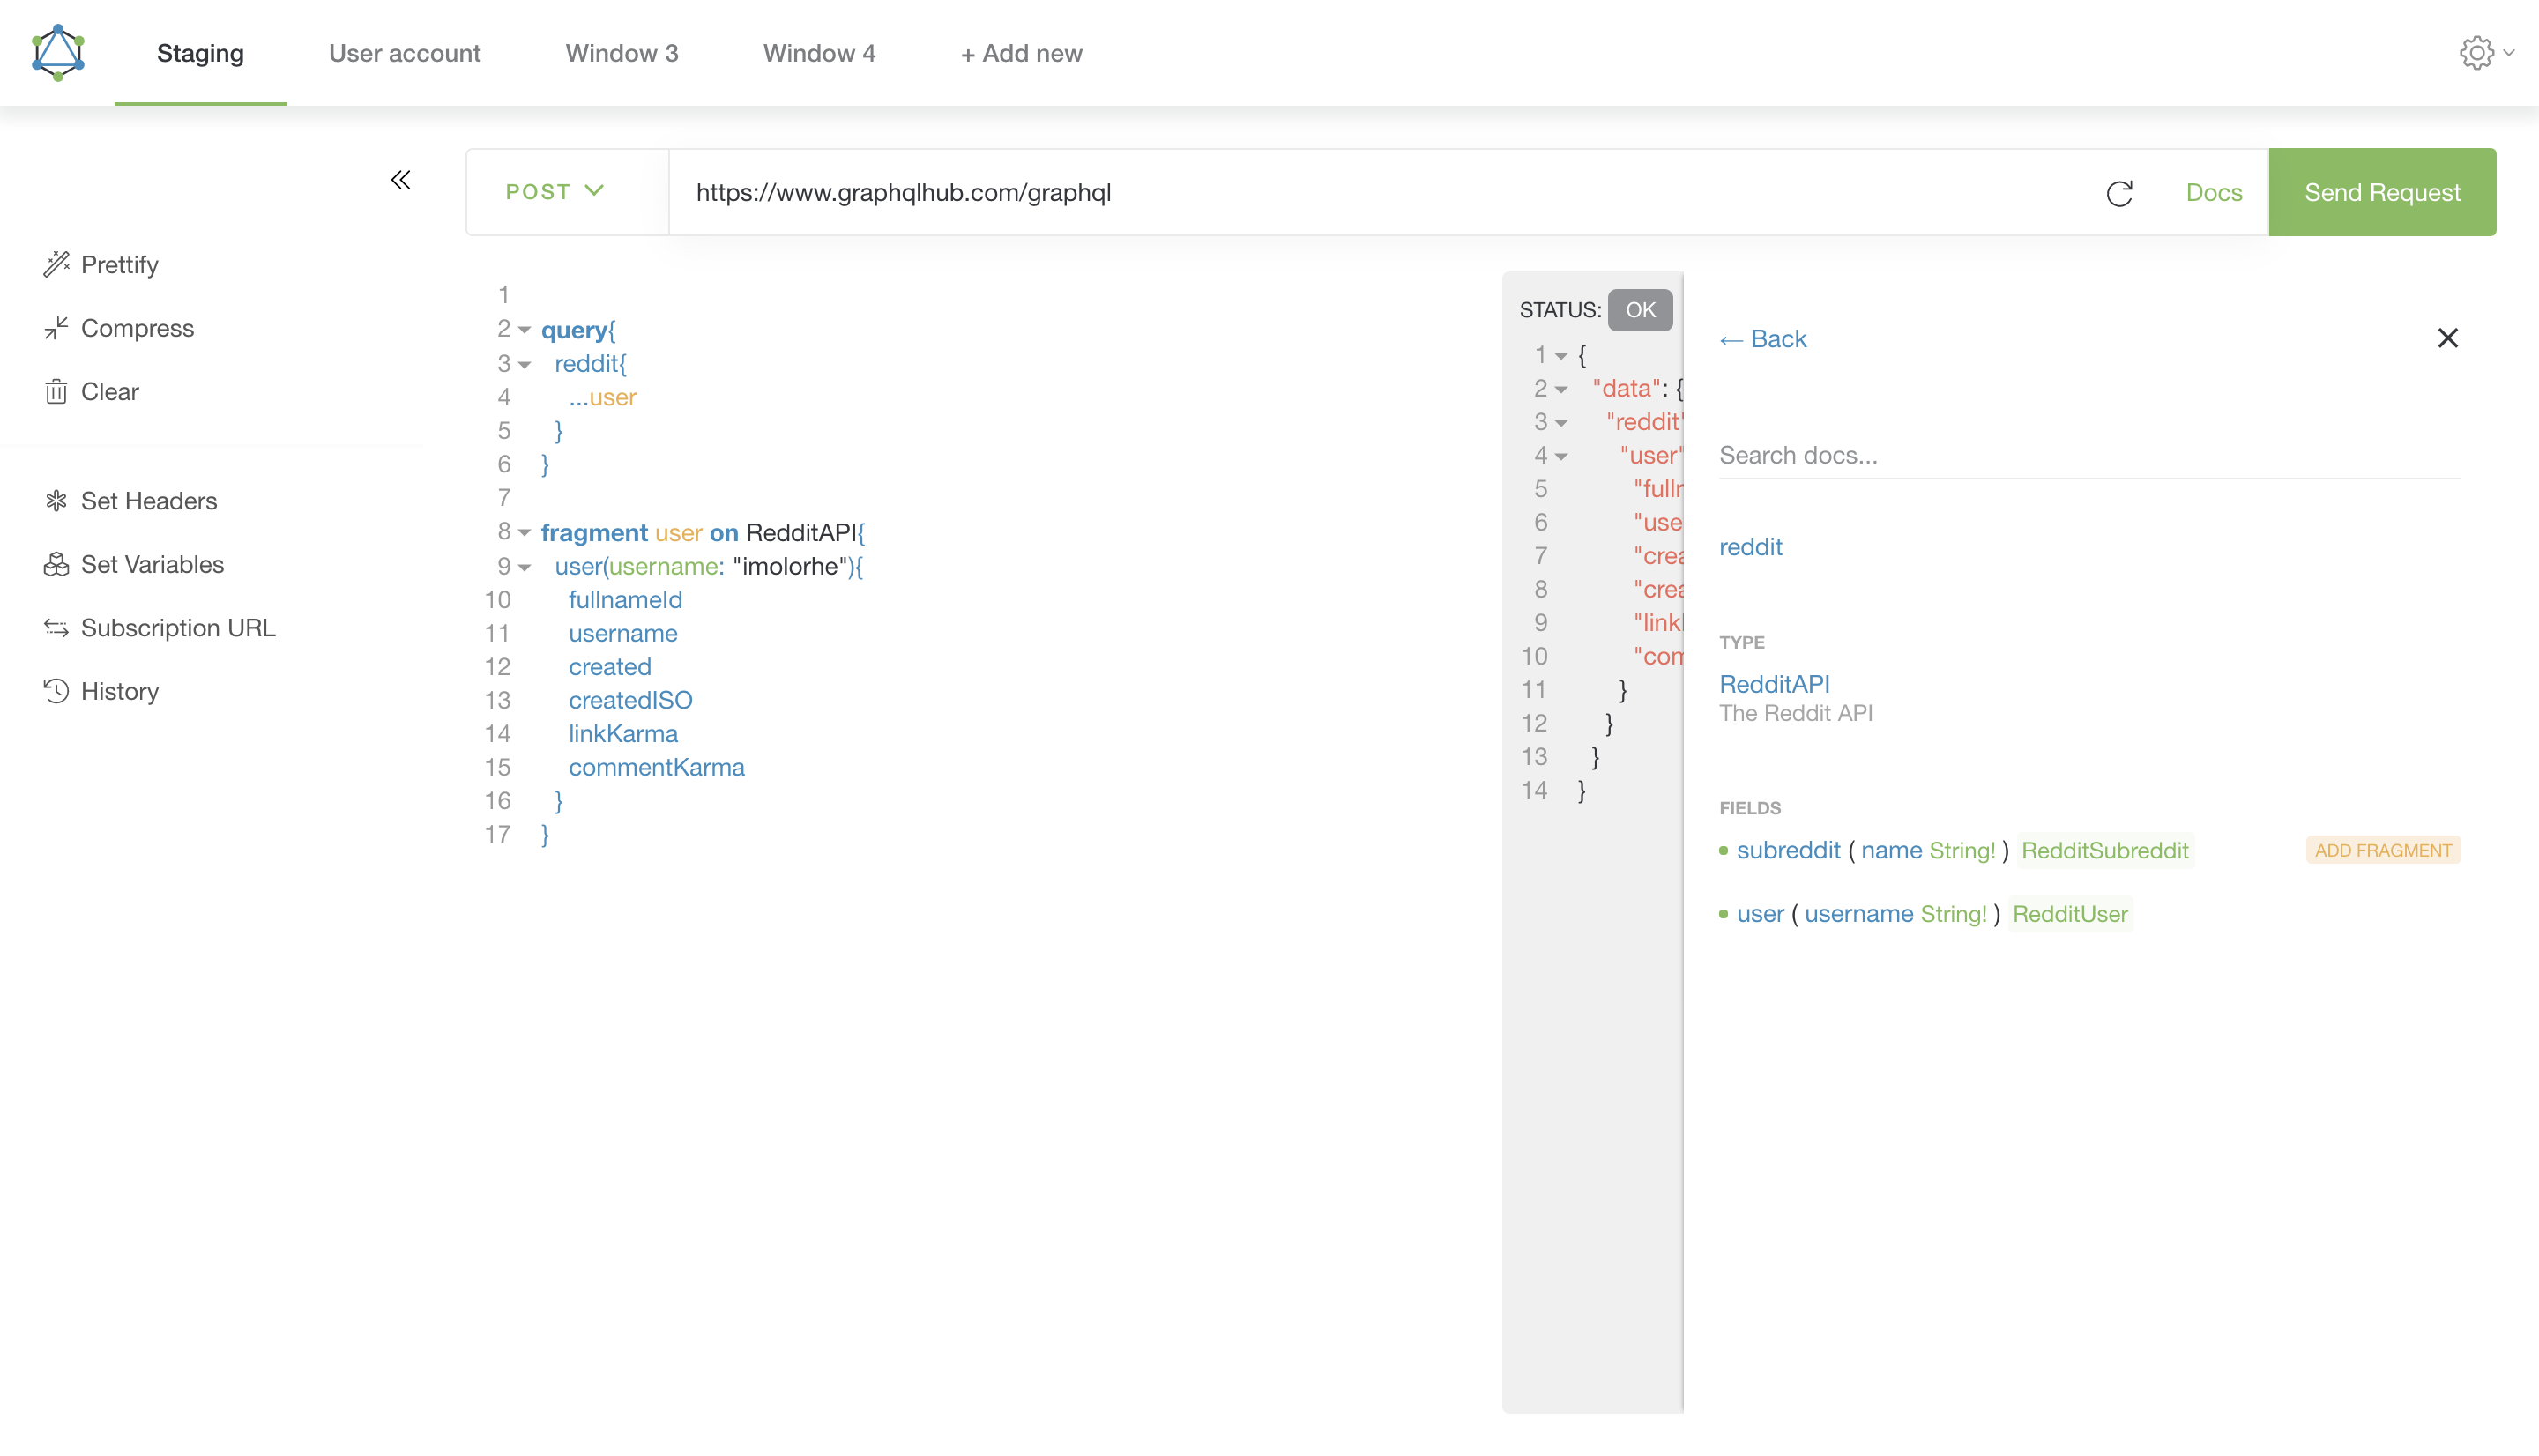
\includegraphics[width=\textwidth]{figures/altair.png}
    \caption[Interfaccia di Altair]{Interfaccia di Altair.
    \label{fig:altair}}
\end{figure}

\subsection{HTTP}
Noto protocollo a livello applicativo per la trasmissione di informazioni in una rete. Il protocollo \ref{itm:http} prevede un'architettura di tipo \textit{client/server}, in cui il \textit{client} esegue una richiesta e il \textit{server} la elabora, fornendo una risposta adeguata.

Una richiesta \ref{itm:http} si compone di quattro parti:
\begin{itemize}
    \item una ``riga di richiesta'' che specifica il tipo di operazione e l'\ref{itm:uri} dell'oggetto della richiesta;
    \item una ``sezione \textit{header}'' in cui vengono fornite informazioni aggiuntive (e.g. credenziali di autenticazione);
    \item una riga vuota che contiene i due caratteri \textit{carriage return} e \textit{line feed};
    \item un \textit{body}, ovvero il corpo del messaggio.
\end{itemize}

Il messaggio di risposta segue una struttura simile, con l'eccezione della riga di richiesta che viene sostituita da una ``riga di stato'',contenente informazioni sul risultato della richiesta sotto forma di codici standard.

Il protocollo HTTP è largamente utilizzato per l'implementazione di \ref{itm:rest}ful \ref{itm:api}; per quanto riguarda il progetto, è stato utilizzato per realizzare l'\ref{itm:api} che si sarebbe interfacciata con il software gestionale del laboratorio di analisi, esponendo determinati \textit{endpoint} per le richieste.

\subsubsection{Insomnia}
\begin{figure}[h!]
    \centering
    
\includegraphics[height=2.5cm]{figures/insomnia.jpg}
    \caption[Logo di Insomnia]{Logo di Insomnia.
    \label{fig:insomnia}}
\end{figure}
Client \textit{open source} e multipiattaforma per \ref{itm:api} GraphQL e \ref{itm:rest}, consente di gestire facilmente lo sviluppo e il testing di richieste HTTP e GraphQL; offre funzionalità di formattazione automatica, variabili d'ambiente e supporto a vari tipi di autenticazione. Insomnia è stato utilizzato per testare gli endpoint delle \ref{itm:api} per il laboratorio di analisi, nonché per sviluppare un client per le \ref{itm:api} del corriere SDA.

\subsection{PostgreSQL}
\begin{figure}[h!]
    \centering
    
\includegraphics[height=2.5cm]{figures/postgres.png}
    \caption[Logo di PostgreSQL]{Logo di PostgreSQL.
    \label{fig:posgres}}
\end{figure}
\ref{itm:dbms} gratuito ed \textit{open source} per la gestione di database relazionali, è considerato uno dei migliori \ref{itm:dbms} gratuiti per la realizzazione di applicazioni web. Oltre alle \textit{feature} di base che condivide con altre soluzioni simili, come l'utilizzo del linguaggio SQL per eseguire query sui dati, PostgreSQL offre delle caratteristiche che risultano molto utili: principalmente offre un sistema di tipi in cui è possibile definire tipi più complessi a partire da quelli di \textit{default} del linguaggio SQL;  permette inoltre l'ereditarietà dei tipi, facilitando un approccio \textit{object-oriented} alla progettazione del database.

PostgreSQL è stato scelto per questo progetto non tanto per le sue caratteristiche peculiari quanto per la sua robustezza e flessibilità; la gestione del database, una volta configurato per funzionare con Rails, è comunque delegata a quest'ultimo.
% $x = 1/\alpha$
% \cite{Eigen1971, Knuth1968}
% $$\zeta = \frac{1039}{\pi}$$


% % For an example of a full page figure, see Fig.~\ref{fig:myFullPageFigure}.


% \texttt{This is a line of code.}


%% Requires fltpage2 package
%%
% \begin{FPfigure}
% 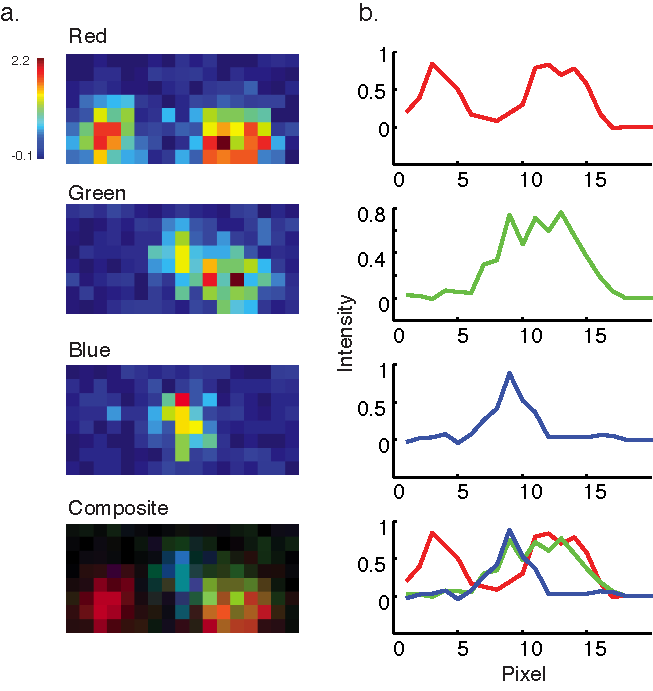
\includegraphics[width=\textwidth]{figures/fullpage}
% \caption[Short figure name.]{This is a full page figure using the FPfigure command. It takes up the whole page and the caption appears on the preceding page. Its useful for large figures. Harvard's rules about full page figures are tricky, but you don't have to worry about it because we took care of it for you. For example, the full figure is supposed to have a title in the same style as the caption but without the actual caption. The caption is supposed to appear alone on the preceding page with no other text. You do't have to worry about any of that. We have modified the fltpage package to make it work. This is a lengthy caption and it clearly would not fit on the same page as the figure. Note that you should only use the FPfigure command in instances where the figure really is too large. If the figure is small enough to fit by the caption than it does not produce the desired effect. Good luck with your thesis. I have to keep writing this to make the caption really long. LaTex is a lot of fun. You will enjoy working with it. Good luck on your post doctoral life! I am looking forward to mine. \label{fig:myFullPageFigure}}
% \end{FPfigure}
% \afterpage{\clearpage}
